\documentclass{beamer}

% Theme and basic packages
\usetheme{Madrid}
\usecolortheme{default}
\usefonttheme{professionalfonts}
\setbeamertemplate{navigation symbols}{}

\usepackage[utf8]{inputenc}
\usepackage[T1]{fontenc}
\usepackage{amsmath, amsfonts, amssymb}
\usepackage{bm}
\usepackage{graphicx}
\usepackage{xcolor}
\usepackage{booktabs}
\usepackage{hyperref}

% Graphics paths
\graphicspath{{eval-figures/}{figures/}}

	itle[Segment Policy Optimization]{Segment Policy Optimization: Segment-Level Credit Assignment for RL in LLMs}
\author{Based on Sections 3--5 of the paper}
\institute{Study Notes}
\date{\today}

\begin{document}

% Title
\begin{frame}
		itlepage
\end{frame}

% Agenda (short)
\begin{frame}{Focus of This Talk}
	\small
	We focus on the mathematical principles in Sections 3--5 only:
	\begin{itemize}
		\item Segment Policy Optimization (SPO): definitions and objectives
		\item Segment-advantage estimation: chain vs tree (Monte Carlo)
		\item Policy optimization with probability masks (clipped surrogate)
		\item Minimal takeaways from experiments, stripped of engineering details
	\end{itemize}
\end{frame}

% Minimal notation
\begin{frame}{Minimal Setup and Notation}
	\small
	Language generation as an MDP with sparse terminal reward:
	\begin{itemize}
		\item State: $s_t = [\boldsymbol x, \boldsymbol y_{<t}]$; action: $a_t = y_t$; deterministic transition $s_{t+1}=[s_t, a_t]$.
		\item Reward: $\mathcal R(\boldsymbol x, \boldsymbol y) \in \{0,1\}$ at episode end; 0 otherwise.
		\item Value: $V(s) = \mathbb E[\sum_t r_t\mid s]$; Advantage: $A(s,a)=V(s')-V(s)$ under deterministic transitions.
	\end{itemize}
	Classical PPO clipped surrogate (for reference):
	\begin{equation*}
		\mathcal{J}_{\text{PPO}}(\theta)
		= \mathbb{E}\Big[ \tfrac{1}{|\boldsymbol y|} \sum_t \min\big( r_t(\theta)\,\hat A_t,\; \mathrm{clip}(r_t,1-\epsilon,1+\epsilon)\,\hat A_t \big) \Big].
	\end{equation*}
\end{frame}

% SPO Overview figure
\begin{frame}{SPO Overview: Segment-Level Credit Assignment}
	\small
	\begin{columns}[T,onlytextwidth]
		\column{0.55\textwidth}
			Key idea: move from trajectory-level or token-level to segment-level.
			\begin{itemize}
				\item Partition $\boldsymbol y=[y_1,\dots,y_T]$ into contiguous segments $\{\text{seg}_k\}_{k=1}^K$.
				\item Define a segment-advantage as an incremental change in $V$ across segment boundaries.
				\item Estimate $V$ via Monte Carlo (critic-free), then optimize a clipped surrogate with masks.
			\end{itemize}
		\column{0.45\textwidth}
			\centering
			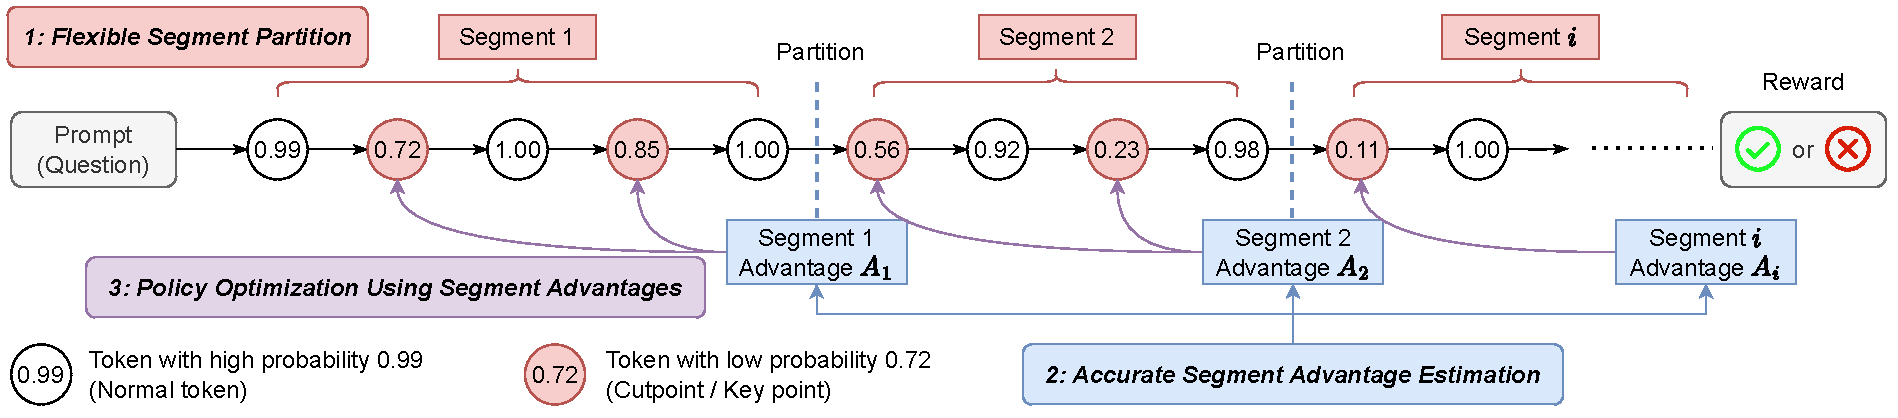
\includegraphics[width=\linewidth]{SPO-framework-short.pdf}
			\vspace{0.3em}
			\footnotesize Overview of SPO components
	\end{columns}
\end{frame}

% Segment definition and advantage
\begin{frame}{Segment and Segment-Advantage}
	\small
	Segment $k$ with boundaries $t_k$ and $t_{k+1}$:
	\[
			ext{seg}_k = [y_{t_k},\dots,y_{t_{k+1}-1}],\qquad \boldsymbol y=[\text{seg}_1,\dots,\text{seg}_K].
	\]
	Segment-level advantage (definition):
	\begin{equation*}
		A_k^{\mathrm{seg}} := V(s_{t_{k+1}}) - V(s_{t_k}) 
		= V([\boldsymbol x, \text{seg}_1,\dots,\text{seg}_k]) - V([\boldsymbol x, \text{seg}_1,\dots,\text{seg}_{k-1}]).
	\end{equation*}
	Remarks:
	\begin{itemize}
		\item Critic-free MC estimation is viable since rewards are Bernoulli; $\mathrm{Var}(\hat V)\le 0.25/N$.
		\item Granularity trades off feedback richness and compute; segment-level balances variance and signal.
	\end{itemize}
\end{frame}

% Partition strategies
\begin{frame}{Partition Strategies (Mathematical View)}
	\small
	Two strategies supported by the framework:
	\begin{itemize}
		\item Fixed token count: split every $M$ tokens.
		\item Cutpoint-based (short CoT): define cutpoints $\mathcal U_\theta=\{t<T\mid \pi_{\theta}(y_t\mid s_t)<\rho\}$;
					given $K$ segments, solve
					\[
						\min_{\{t_k\}} \sum_{k=1}^K \big|\mathcal U_\theta\cap[t_k, t_{k+1})\big|^2
					\]
					whose minimizer evenly distributes cutpoints across segments, i.e.,
					$\big|\mathcal U_\theta\cap[t_k,t_{k+1})\big|=|\mathcal U_\theta|/K$.
	\end{itemize}
	\vspace{0.3em}
	\centering
	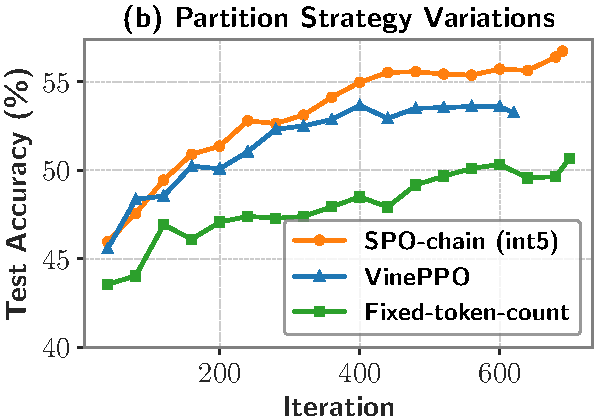
\includegraphics[width=0.78\linewidth]{Segment-methods-var.pdf}
\end{frame}

% Chain-based MC
\begin{frame}{Chain-Based MC Estimation of $V$}
	\small
	For boundary state $s_{t_k}$, sample $N$ rollouts $\boldsymbol\tau^{(j)}_{t_k}\sim\pi_\theta(\cdot\mid s_{t_k})$ and estimate
	\[
		\hat V(s_{t_k})=\tfrac{1}{N}\sum_{j=1}^N \mathcal R\big(\boldsymbol x, [\boldsymbol y_{<t_k},\,\boldsymbol\tau^{(j)}_{t_k}]\big),\quad 
		\hat A_k^{\mathrm{seg}}=\hat V(s_{t_{k+1}})-\hat V(s_{t_k}).
	\]
	\vspace{0.4em}
	Training objective with probability masks (focus on low-probability tokens):
	\begin{equation*}
	\small
	\begin{aligned}
	\mathcal{J}_{\text{SPO}}^{\text{chain}}(\theta)
	&= \mathbb{E}\Big[\, \tfrac{1}{Z}\sum_{k=1}^K \sum_{t=t_k}^{t_{k+1}-1} M_t\cdot \min\big(r_t\hat A_k^{\mathrm{seg}},\;\mathrm{clip}(r_t,1-\epsilon,1+\epsilon)\hat A_k^{\mathrm{seg}}\big) \\
	&\qquad\qquad - \beta\, D_{\mathrm{KL}}(\pi_\theta\Vert\pi_{\mathrm{ref}})\,\Big],\quad M_t=\mathbb I\big(\pi_{\theta_{\mathrm{old}}}(a_t\mid s_t)<\rho\big).
	\end{aligned}
	\end{equation*}
	\vspace{-0.3em}
	\centering
	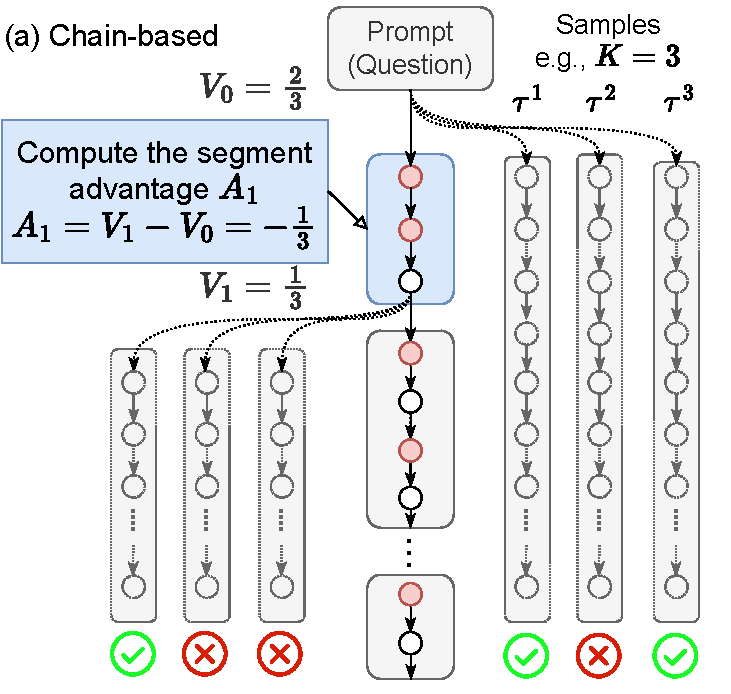
\includegraphics[width=0.78\linewidth]{SPO-chain-short.pdf}
\end{frame}

% Tree-based MC
\begin{frame}{Tree-Based MC: Reusing Samples Efficiently}
	\small
	Model sampling as a tree. For node $n$ with history $\operatorname{hist}(n)$ and segment $\operatorname{seg}(n)$ of $M$ tokens:
	\[
		\hat V(n)= \begin{cases}
			\mathcal R(\boldsymbol x, \operatorname{hist}(n)), & n\text{ is leaf}\\
				frac{1}{|\operatorname{Ch}(n)|}\sum_{n'\in\operatorname{Ch}(n)} \hat V(n'), & \text{otherwise}
		\end{cases}
	\]
	Advantage within sibling group:
	\[
		\hat A(n)=\hat V(n)-\operatorname{mean}_{n'\in\operatorname{Sib}(n)}\hat V(n')\quad \text{or}\quad \frac{\hat V(n)-\operatorname{mean}}{\operatorname{std}}.
	\]
	Training objective (masked tokens, non-zero advantages):
	\begin{equation*}
	\small
	\begin{aligned}
	\mathcal J_{\text{SPO}}^{\operatorname{tree}}(\theta)
	&= \mathbb E\Big[\, \tfrac{1}{Z}\sum_{n: \hat A(n)\neq 0}\sum_{t=1}^{|\operatorname{seg}(n)|} M_{n,t}\cdot \min\big(r_{n,t}\hat A(n),\;\mathrm{clip}(r_{n,t},1-\epsilon,1+\epsilon)\hat A(n)\big) \\
	&\qquad\qquad - \beta\, D_{\mathrm{KL}}(\pi_\theta\Vert\pi_{\mathrm{ref}})\,\Big].
	\end{aligned}
	\end{equation*}
	\vspace{-0.5em}
	\centering
	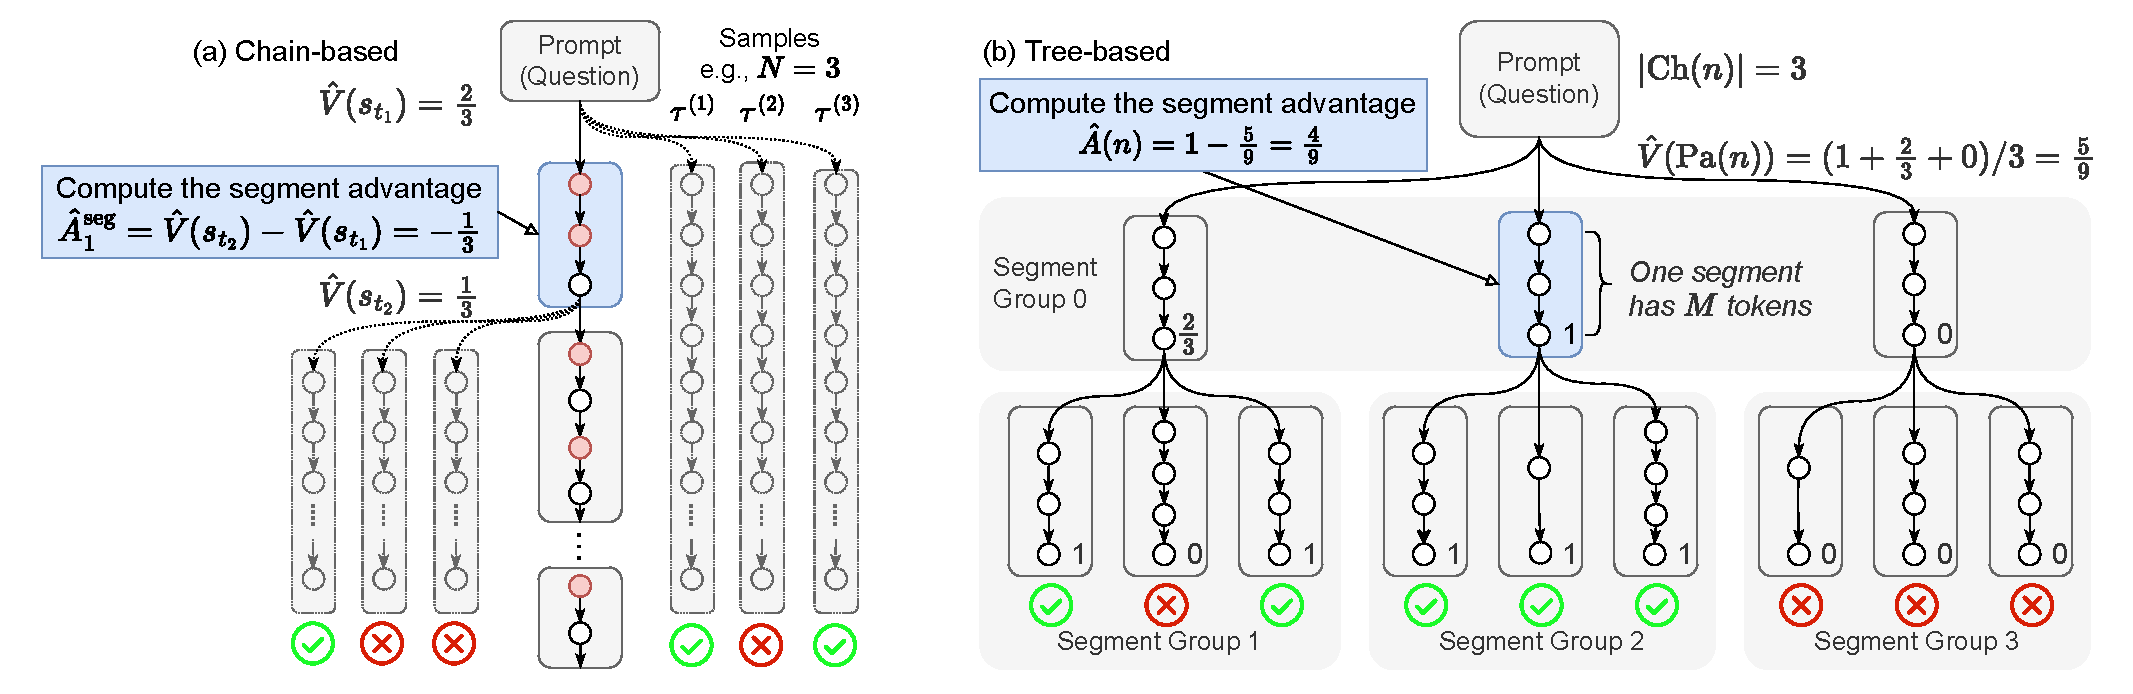
\includegraphics[width=0.78\linewidth]{SPO-framework-both.pdf}
\end{frame}

% Intuitions and trade-offs (math-centric)
\begin{frame}{Why Segment-Level Works (Math Intuition)}
	\small
	\begin{itemize}
		\item Signal-to-Noise: $\hat V$ is Bernoulli-MC; segment-level differences $\Delta V$ provide concentrated signals at boundary changes.
		\item Bias–Variance: token-level needs a critic (bias risk); trajectory-level has sparse credit; segment-level balances both.
		\item Masking focuses gradient on low-probability tokens that drive $\Delta V$, reducing loss on near-deterministic tokens.
		\item Tree reuses samples: bottom-up $\hat V$ aggregation reduces sample complexity while supplying many training segments.
	\end{itemize}
\end{frame}

% Minimal experiment-backed evidence (no engineering details)
\begin{frame}{Evidence Snapshot (Theory-Oriented View)}
	\small
	\begin{columns}[T,onlytextwidth]
		\column{0.5\textwidth}
			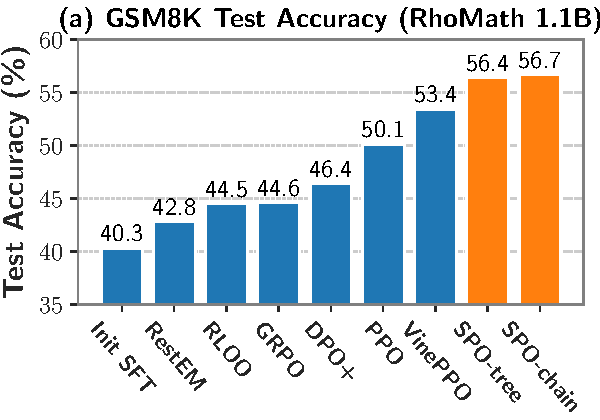
\includegraphics[width=\linewidth]{GSM8K-acc-only-bar.pdf}\\[-0.6em]
			\footnotesize Segment-level advantages outperform trajectory-level baselines.
		\column{0.5\textwidth}
			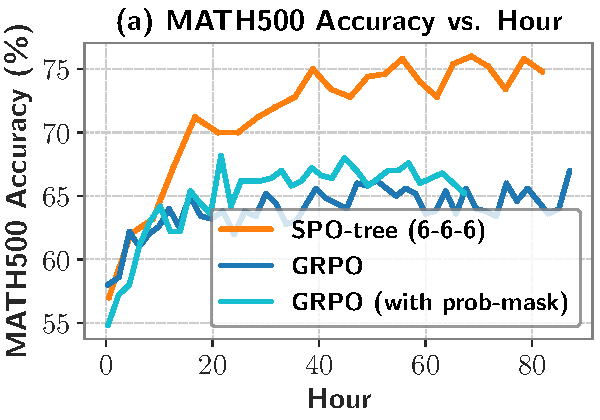
\includegraphics[width=\linewidth]{SPO-tree-GRPO-line-LoT.pdf}\\[-0.6em]
			\footnotesize Tree-based advantages improve accuracy under same wall-clock.
	\end{columns}
\end{frame}

% Conclusion
\begin{frame}{Conclusions (Sections 3--5)}
	\small
	\begin{itemize}
		\item Define segment-advantages $A_k^{\mathrm{seg}}=V(s_{t_{k+1}})-V(s_{t_k})$ and estimate $V$ via MC (critic-free).
		\item Chain vs tree estimators: tree yields higher sample efficiency via reuse and group-wise advantages.
		\item Optimize with clipped surrogate and token-probability masks to sharpen credit assignment.
		\item Segment granularity and tree width/depth control the bias–variance–compute trade-offs.
	\end{itemize}
\end{frame}

\end{document}
